% !TEX root = ../BeamerTemplate.tex
%%%%%%%%%%%%%%%%%%%%%%%%%%%%%%%%%%%%%%%%%%%%%%%%%%%%%%%%%%%%%%%%%%%%%%%%%%%%%%%%%%

% This divider is intentionally placed after the Thank You slide. Add any
% supplementary or backup frames below it; they remain outside the main-frame
% count because \appendix is activated by AuxiliaryFiles/SettingBackup.tex.
{\setbeamercolor{background canvas}{bg=Blue}
\begingroup
\setbeamertemplate{navigation symbols}{}
\begin{frame}[plain,noframenumbering]\label{Appendix}
  \centering
  \color{white}
  \vfill
  {\bfseries\Huge Appendix}\par
  \vspace{0.35cm}
  {\Large Supplementary Material}\par
  \vfill
  {\small Muhammad Zharfan Wiranata\\
  National Sun Yat-sen University}
  \vfill
\end{frame}



\endgroup}

\begin{frame}{Why Simulation Was Prioritized}
  \begin{itemize}
    \item Experimental fabrication was postponed due to cost constraints and
          fabrication-yield considerations.
    \item Fabrication and experimental verification are planned for the
          mid-to-upper FR3 band.
  \end{itemize}

  \begin{block}{Current Thesis Scope}
    Therefore, this thesis focuses on simulation-based design and performance
    evaluation.
  \end{block}
\end{frame}




% Add further appendix frames below this line.
\begin{frame}{Simulation-Based Thesis Methodology}{Experimental Validation as Future Work}
  \begin{block}{Simulation Method}
    \begin{itemize}
      \item \textbf{EM design:} The unit cell, patch antenna, and
            $20\!\times\!20$ transmitarray lensZZ
            were designed and characterized in Ansys HFSS at 38~GHz.
      \item \textbf{Channel validation:} The end-to-end MIMO channel was
            reconstructed and cross-validated
            using HFSS SBR+, HFSS Hybrid, and Sionna-RT.
      \item \textbf{System evaluation:} Performance was evaluated in Sionna-RT
            through paired
            Monte Carlo trials of the with-lens and without-lens configurations.
    \end{itemize}
  \end{block}

  % \begin{block}{Experimental Scope}
  %   Fabrication and measurement were deferred because of cost constraints and
  %   the expected fabrication yield. Experimental validation in the mid-to-upper
  %   FR3 band remains an important next step.
  % \end{block}
\end{frame}

% Add further appendix frames below this line.
\begin{frame}{Constructing the MIMO Channel in Sionna-RT}
\scriptsize
\begin{columns}[T,onlytextwidth]
  \column{0.49\textwidth}
  \begin{block}{1. One RX angle per simulation}
    \begin{itemize}
      \setlength{\itemsep}{0.2em}
      \item For angle $\theta_i$, HFSS
            \texttt{GainTheta}/\texttt{GainPhi} and
            \texttt{rETheta}/\texttt{rEPhi} form one complex RX pattern.
      \item Sionna-RT supports only one angle-specific RX radiation pattern per
            run. Therefore, each RX pattern is simulated separately with all
            $N$ TX elements.
    \end{itemize}
    \[
      \theta_i \;\longrightarrow\;
      \mathbf{h}_i(f)=
      \bigl[H_{i1}(f),\ldots,H_{iN}(f)\bigr]
    \]
    Each run therefore produces one canonical channel row.
  \end{block}

  \column{0.49\textwidth}
  \begin{block}{2. Stack all RX-angle results}
    Repeat the simulation for $i=1,\ldots,N$, then stack the resulting rows:
    \[
      \mathbf{H}(f)=
      \left[\begin{array}{c}
        \mathbf{h}_1(f)\\[-0.15em]
        \mathbf{h}_2(f)\\[-0.15em]
        \vdots\\[-0.15em]
        \mathbf{h}_N(f)
      \end{array}\right]
      \in\mathbb{C}^{N\times N}.
    \]
    For a $3\!\times\!3$ channel, three angle-specific RX simulations produce
    the three rows of $\mathbf{H}(f)$.
  \end{block}
\end{columns}

\vspace{0.10cm}
\begin{beamercolorbox}[rounded=true,sep=0.8ex,wd=\linewidth]{takeaway}
  \centering
  \textbf{One run: $1$ RX pattern $\times$ $N$ TXs}
  $\;\Longrightarrow\;$
  \textbf{$N$ RX-angle runs: one constructed $N\!\times\!N$ MIMO channel.}
\end{beamercolorbox}
\end{frame}


\begin{frame}{Spatial Decorrelation Using the Center TX}
\scriptsize
\begin{columns}[T,onlytextwidth]
  \column{0.43\textwidth}
  \begin{block}{Fixed-reference construction}
    \centering
    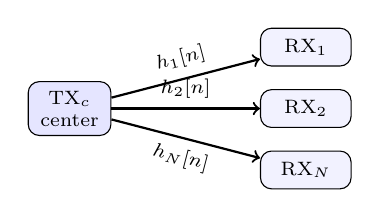
\begin{tikzpicture}[
      tx/.style={draw,rounded corners,fill=Blue!10,minimum width=1.05cm,
                 minimum height=0.55cm,align=center},
      rx/.style={draw,rounded corners,fill=Blue!5,minimum width=1.15cm,
                 minimum height=0.48cm,align=center},
      every node/.style={font=\scriptsize}
    ]
      \node[tx] (tx) at (0,0) {$\mathrm{TX}_{c}$\\center};
      \node[rx] (rx1) at (3.0,0.78) {$\mathrm{RX}_{1}$};
      \node[rx] (rx2) at (3.0,0.00) {$\mathrm{RX}_{2}$};
      \node[rx] (rxn) at (3.0,-0.78) {$\mathrm{RX}_{N}$};
      \draw[->,thick] (tx)--node[above,sloped] {$h_1[n]$} (rx1);
      \draw[->,thick] (tx)--node[above] {$h_2[n]$} (rx2);
      \draw[->,thick] (tx)--node[below,sloped] {$h_N[n]$} (rxn);
    \end{tikzpicture}

    \vspace{0.10cm}
    Fix one center transmitter and collect
    $h_i[n]=H_{i,c}[n]$ for every RX branch $i$.
    The center branches are $\mathrm{TX}_2$, $\mathrm{TX}_3$, and
    $\mathrm{TX}_5$ for $N=3,5,9$ (zero-based $c=1,2,4$).
  \end{block}

  \column{0.54\textwidth}
  \begin{block}{Pairwise RX correlation and decorrelation}
    For each RX pair $(i,j)$, the complex center-TX responses are compared using
    \begin{align*}
      \rho_{ij}&=
      \frac{\sum_n h_i[n]h_j^*[n]}
      {\sqrt{\left(\sum_n|h_i[n]|^2\right)
                   \left(\sum_n|h_j[n]|^2\right)}} ,\\[-0.15em]
      D_{ij}&=1-|\rho_{ij}|.
    \end{align*}
    \textbf{$D_{ij}\approx0$:} similar/correlated RX responses.\par\smallskip
    \textbf{$D_{ij}\approx1$:} distinct/decorrelated RX responses.\par\smallskip
    All RX pairs are summarized using global pooling or a typical local-block
    median.
  \end{block}
\end{columns}

\vspace{0.10cm}
\begin{beamercolorbox}[rounded=true,sep=0.8ex,wd=\linewidth]{takeaway}
  \textbf{Why the center TX?} A fixed source isolates differentiation among RX
  angle/pattern responses. This single-TX metric is not the singular-value
  structure of the full constructed $N\!\times\!N$ MIMO channel.
\end{beamercolorbox}
\end{frame}


\begin{frame}{Worked Example: Center-TX Decorrelation}
\scriptsize
\begin{columns}[T,onlytextwidth]
  \column{0.37\textwidth}
  \begin{block}{Example $3\!\times\!3$ channel}
    Select the center element, $\mathrm{TX}_2$, and observe two channel samples
    from this TX to each RX:
    \[
      \begin{array}{c|c}
        \text{RX branch} & \mathbf h_i=[h_i[1],h_i[2]]\\ \hline
        \mathrm{RX}_1 & [1,\,j]\\
        \mathrm{RX}_2 & [2,\,2j]\\
        \mathrm{RX}_3 & [1,\,-j]
      \end{array}
    \]
    Here, $\mathbf h_2=2\mathbf h_1$: its magnitude is larger, but its
    normalized response has the same shape and phase progression.
  \end{block}

  \column{0.60\textwidth}
  \begin{block}{RX$_1$--RX$_2$: fully correlated}
    \begin{align*}
      \rho_{12}
      &=\frac{1(2)^*+j(2j)^*}
      {\sqrt{(1+1)(4+4)}}
      =\frac{2+2}{4}=1,\\[-0.2em]
      D_{12}&=1-|\rho_{12}|=0.
    \end{align*}
  \end{block}

  \begin{block}{RX$_1$--RX$_3$: fully decorrelated}
    \begin{align*}
      \rho_{13}
      &=\frac{1(1)^*+j(-j)^*}
      {\sqrt{(1+1)(1+1)}}
      =\frac{1-1}{2}=0,\\[-0.2em]
      D_{13}&=1-|\rho_{13}|=1.
    \end{align*}
  \end{block}
\end{columns}

\vspace{-0.07cm}
\begin{beamercolorbox}[rounded=true,sep=0.6ex,wd=\linewidth]{takeaway}
  \centering
  $D_{12}=0$, $D_{13}=1$, and similarly $D_{23}=1$.
  \textbf{The metric measures normalized channel similarity; amplitude scaling
  alone does not create decorrelation.}
\end{beamercolorbox}
\end{frame}



% -----------------------------------------------------------------------------
% Evaluation-equation reference slides
% -----------------------------------------------------------------------------

\begin{frame}[t]{Evaluation Equations I: Channel Construction}
  \footnotesize
  \begin{columns}[T,onlytextwidth]
    \begin{column}{0.49\textwidth}
      \begin{block}{Canonical frequency-domain channel}
        \begin{equation*}
          \mathbf H(f)=\bigl[H_{ij}(f)\bigr]
          \in\mathbb C^{N_R\times N_T}
        \end{equation*}
        \vspace{-1.5ex}
        \begin{equation*}
          \mathbf y(f)=\mathbf H(f)\mathbf x(f)+\mathbf n(f)
        \end{equation*}
      \end{block}

      \begin{block}{Sionna-RT channel coefficient}
        \begin{equation*}
          H_{ij}(f)=\sum_{\ell=1}^{L_{ij}}
          \alpha_{ij,\ell}e^{-j2\pi f\tau_{ij,\ell}}
        \end{equation*}
        \scriptsize $\alpha_{ij,\ell}$ and $\tau_{ij,\ell}$ are the complex
        gain and delay of path $\ell$.
      \end{block}
    \end{column}

    \begin{column}{0.49\textwidth}
      \begin{block}{Singular-value decomposition}
        \begin{equation*}
          \mathbf H=\mathbf U\boldsymbol\Sigma\mathbf V^{H},\qquad
          \boldsymbol\Sigma=\operatorname{diag}(\sigma_1,\ldots,\sigma_q)
        \end{equation*}
        \vspace{-1ex}
        \begin{equation*}
          \sigma_1\geq\cdots\geq\sigma_q\geq0,\qquad
          q=\min(N_R,N_T)
        \end{equation*}
      \end{block}

      \begin{block}{Power-independent channel structure}
        \begin{equation*}
          \widetilde{\mathbf H}
          =\frac{\mathbf H}{\lVert\mathbf H\rVert_{\mathrm F}},\qquad
          \lVert\mathbf H\rVert_{\mathrm F}^{2}
          =\sum_{i,j}|H_{ij}|^2
        \end{equation*}
      \end{block}
    \end{column}
  \end{columns}

  \MethodNote{Raw $\mathbf H$ retains absolute link gain; $\widetilde{\mathbf H}$
  isolates the relative distribution of power among spatial modes.}
\end{frame}


\begin{frame}[t]{Evaluation Equations II: Link Budget and Outage}
  \footnotesize
  \begin{columns}[T,onlytextwidth]
    \begin{column}{0.57\textwidth}
      \begin{block}{Non-coherent combination of simultaneous TX branches}
        \begin{align*}
          P_{\mathrm{RX}}(f)
            &=P_{\mathrm{TX}}\sum_{i=1}^{N_T}|H_i(f)|^2,\\
          P_{\mathrm N}
            &=kTB\,10^{\mathrm{NF}/10},\\
          \gamma(f)
            &=\frac{P_{\mathrm{RX}}(f)}{P_{\mathrm N}}.
        \end{align*}
      \end{block}
    \end{column}

    \begin{column}{0.41\textwidth}
      \begin{block}{Equivalent-SISO link capacity}
        \begin{equation*}
          C_{\mathrm{link}}
          =\frac{1}{N_f}\sum_{m=1}^{N_f}
          \log_2\!\left(1+\gamma(f_m)\right)
        \end{equation*}
        \centering\scriptsize bit/s/Hz
      \end{block}

      \begin{block}{Empirical outage probability}
        \begin{equation*}
          P_{\mathrm{out}}(C_{\mathrm{th}})
          =\frac{1}{N_{\mathrm{obs}}}
          \sum_{u=1}^{N_{\mathrm{obs}}}
          \mathbf 1\!\left\{C_u<C_{\mathrm{th}}\right\}
        \end{equation*}
      \end{block}
    \end{column}
  \end{columns}

  \begin{beamercolorbox}[rounded=true,sep=0.4ex,wd=\linewidth]{caution}
    \scriptsize\textbf{Caution:} $C_{\mathrm{link}}$ retains absolute gain;
    fixed-SNR $C_{\mathrm{MIMO}}$ measures channel structure. The
    1~bit/s/Hz threshold yielded 0\% outage.
  \end{beamercolorbox}
\end{frame}


\begin{frame}[t]{Evaluation Equations III: Conditioning and Effective Rank}
  \footnotesize
  \begin{columns}[T,onlytextwidth]
    \begin{column}{0.48\textwidth}
      \begin{block}{Condition number}
        \begin{equation*}
          \kappa=\frac{\sigma_1}{\sigma_q},\qquad
          \kappa_{\mathrm{dB}}=20\log_{10}\kappa
        \end{equation*}
      \end{block}

      \begin{center}
        \begin{tabular}{c@{\quad$\Longrightarrow$\quad}l}
          $\kappa\rightarrow1$ & balanced modes\\[0.5ex]
          $\kappa\gg1$ & ill-conditioned channel
        \end{tabular}
      \end{center}
    \end{column}

    \begin{column}{0.50\textwidth}
      \begin{block}{Singular-value power fractions}
        \begin{equation*}
          p_i=\frac{\sigma_i^2}{\sum_{k=1}^{q}\sigma_k^2},
          \qquad \sum_{i=1}^{q}p_i=1
        \end{equation*}
      \end{block}

      \begin{block}{Entropy-based effective rank}
        \begin{equation*}
          r_{\mathrm{eff}}
          =\operatorname{exp}\!\left(-\sum_{i=1}^{q}p_i\ln p_i\right),
          \qquad 1\leq r_{\mathrm{eff}}\leq q
        \end{equation*}
      \end{block}
    \end{column}
  \end{columns}

  \Takeaway{Favorable multiplexing has a smaller $\kappa$ and a larger
  $r_{\mathrm{eff}}$. Both depend on singular-value ratios and are unchanged by
  Frobenius normalization.}
\end{frame}


\begin{frame}[t]{Evaluation Equations IV: Spatial Correlation and Decorrelation}
  \scriptsize
  \begin{columns}[T,onlytextwidth]
    \begin{column}{0.50\textwidth}
      \begin{block}{Full-matrix normalized correlation}
        \begin{align*}
          \mathbf R_{\mathrm{RX}}
          &=\mathbf D_{\mathrm{RX}}^{-1/2}
            \mathbf H\mathbf H^H
            \mathbf D_{\mathrm{RX}}^{-1/2},\\
          \mathbf R_{\mathrm{TX}}
          &=\mathbf D_{\mathrm{TX}}^{-1/2}
            \mathbf H^H\mathbf H
            \mathbf D_{\mathrm{TX}}^{-1/2},
        \end{align*}
        where
        \begin{equation*}
          \mathbf D_{\mathrm{RX}}=\operatorname{diag}(\mathbf H\mathbf H^H),
          \quad
          \mathbf D_{\mathrm{TX}}=\operatorname{diag}(\mathbf H^H\mathbf H).
        \end{equation*}
      \end{block}

      Off-diagonal magnitudes quantify response similarity; smaller values
      indicate greater spatial independence.
    \end{column}

    \begin{column}{0.48\textwidth}
      \begin{block}{Pairwise CFR correlation}
        \begin{equation*}
          \rho_{ij}=\frac{\sum_n h_i[n]h_j^*[n]}
          {\sqrt{\left(\sum_n|h_i[n]|^2\right)
          \left(\sum_n|h_j[n]|^2\right)}}
        \end{equation*}
        \vspace{-1.5ex}
        \begin{equation*}
          D_{ij}=1-|\rho_{ij}|,\qquad 0\leq D_{ij}\leq1
        \end{equation*}
      \end{block}

      \begin{block}{Typical-block and amplitude-sensitive summaries}
        \begin{align*}
          D_{ij}^{\mathrm{med}}
            &=1-\operatorname{median}_{w,t}|\rho_{ij}^{(w,t)}|,\\
          Q_{ij}^{\mathrm{raw}}
            &=\frac{1}{N_s}\sum_n|h_i[n]-h_j[n]|^2.
        \end{align*}
      \end{block}
    \end{column}
  \end{columns}

\end{frame}


\begin{frame}[t]{Evaluation Equations V: MIMO Capacity and Scaling}
  \footnotesize
  \begin{columns}[T,onlytextwidth]
    \begin{column}{0.59\textwidth}
      \begin{block}{Equal-power MIMO capacity}
        \begin{align*}
          C_{\mathrm{MIMO}}(\gamma)
          &=\mathbb E_f\!\left[
            \log_2\det\!\left(
              \mathbf I_{N_R}+\frac{\gamma}{N_T}
              \mathbf H\mathbf H^H
            \right)\right]\\
          &=\mathbb E_f\!\left[
            \sum_{i=1}^{q}\log_2\!\left(
              1+\frac{\gamma}{N_T}\sigma_i^2(f)
            \right)\right].
        \end{align*}
      \end{block}
    \end{column}

    \begin{column}{0.39\textwidth}
      \begin{block}{Per-dimension efficiency}
        \begin{equation*}
          \eta_r(N)=\frac{r_{\mathrm{eff}}}{N},
          \qquad
          \eta_C(N)=\frac{C_{\mathrm{MIMO}}}{N}
        \end{equation*}
      \end{block}

      \begin{block}{Operating points in this thesis}
        \scriptsize
        Chapter 2 solver comparison: 20~dB.\\[0.5ex]
        Chapter 3 constructed channels: fixed normalized 10~dB.\\[0.5ex]
        Order study: $N=3,5,9$.
      \end{block}
    \end{column}
  \end{columns}

  \Takeaway{Absolute capacity measures total supported rate; $\eta_r$ and
  $\eta_C$ measure per-dimension use. These are ideal Shannon bounds, not coded
  throughput.}
\end{frame}
